\documentclass[12pt, a4paper]{article}

%%%%%%%%%%%%%%%%%%%%%%%%%%%%%%%%%%%%%% PACKAGES %%%%%%%%%%%%%%%%%%%%%%%%%%%%%%%%
\usepackage[swedish]{babel}
\usepackage[utf8]{inputenc}
\usepackage[hidelinks]{hyperref}
\usepackage{
  amsmath,
  amssymb,
  caption,
  color,
  float,
  graphicx,
  listings,
  siunitx,
  tikz,
  parskip,
  pdflscape,
  pgfgantt,
  scrextend,
}

\usetikzlibrary{positioning}

%%%%%%%%%%%%%%%%%%%%%%%%%%%%%%%  NICE PALETTE  %%%%%%%%%%%%%%%%%%%%%%%%%%%%%%%%%

% https://images.squarespace-cdn.com/content/v1/638773c92dfb4812d5f5ff28/1669823793535-UWL204TLLHME6SFDP2QZ/image-asset.png
\definecolor{navy}{RGB}{16,37,38}
\definecolor{ginger}{RGB}{205,126,89}
\definecolor{seafoam}{RGB}{69,115,115}
\definecolor{sunflower}{RGB}{221,178,71}
\definecolor{jean}{RGB}{90,104,104}

%%%%%%%%%%%%%%%%%%%%%%%%%%%%%%%%%  TITLE PAGE  %%%%%%%%%%%%%%%%%%%%%%%%%%%%%%%%%

\title{Projektplan - Binäranalys med en hybrid av automatiska och manuella metoder}
\author{
    Albin Otterhäll \and
    Clara Salberg \and
    Enayatullah Norozi \and
    Linus Wallman \and
    Loke Gustafsson \and
    Samuel Kyletoft
}
\date{2023-02-10}

%%%%%%%%%%%%%%%%%%%%%%%%%%%%% DOCUMENT STRUCTURE %%%%%%%%%%%%%%%%%%%%%%%%%%%%%%%

\begin{document}

%%%%%%%%%%%%%%%%%%%%%%%%%%%%%%%%  PROJECT NAMES  %%%%%%%%%%%%%%%%%%%%%%%%%%%%%%%
%
\newcommand{\stoe}{S$^2$E}

\maketitle

\newpage

% TODO remove this for final report
\newpage

\tableofcontents
\newpage

\addcontentsline{toc}{section}{Begreppslista}
\section*{Begreppslista}
\begin{labeling}{begreppslista}

  \item [\textbf{Black-box}] Analys av ett objekt som endast betraktar dess
      yttre utseende och beteende, till skillnad från white-box-analys som även
      betraktar vad som händer inuti.

  \item [\textbf{Concolic testing}] En sorts fuzztesting där indata genereras
      genom att med en SMT-lösare lösa ekvationerna som beskriver en körning som
      ursprungligen följer körningen för en seed-indata, men vid ett angivet
      hopp avviker. Detta är en effektiv metod för att konstruera indata som tar
      speciella svår-tagna hopp.

  \item [\textbf{ELF}] \emph{Executable and Linkable Format}. Filformatet för
      exekverbara filer på Unix.

  \item [\textbf{Fuzzing}] Att slumpmässigt generera indata till ett system i
      ett försök att hitta buggar eller genom frånvaron av dåligt beteende
      betryggas i systemets kvalité. Vissa fuzztestmotorer genererar ny indata
      med genetiska algoritmer och vissa använder white-box binärinstrumentation
      för att evaluera indata.

  \item [\textbf{QEMU}] Ett välunderhållet öppen källkods emulatorramverk med stöd
    för många plattformar och som stöder både user-space emulering av en process
    samt emulering av ett helt system.

  \item [\textbf{\stoe}] \stoe, eller \emph{The Selective Symbolic Execution Platform}, är
      en platform som tillhandahåller symbolisk exekvering inuti den virtuella
      maskinen QEMU.

  \item [\textbf{SMT Solver}] En Satisfiability modulo theories-lösare är ett
      program som kan lösa ekvationssystem för olika matematiska objekt. Exempel
      på teorier är modulär aritmetik eller bitvektorer. En SMT-lösare kan till
      exempel lösa ekvationer konstruerade i symbolisk exekvering.

  \item [\textbf{Symbolisk exekvering}] Att tilldela variabler symboliska, i
      motsats till konkreta, värden under programmets exekvering. Med denna
      analysteknik kan enskilda körningar ge information som annars hade krävt
      en uttömmande sökning.

\end{labeling}


\newpage

\section{Bakgrund}
% BAKGRUNDENS UPPGIFT?: Motivera behovet att visualiseringsverktyg för fuzzing
% (fuzzing används slarvigt, inkludera tex concolic testing)

Att läsa källkod är ett sätt att förstå program, men ibland är det gynnsamt att istället betrakta
maskinkoden direkt. Detta kan vara för att
\begin{itemize}
  \item utesluta påverkan av kompilatorbuggar som ger oväntad maskinkod
  \item se hur UB (\emph{undefined behaviour}) har utnyttjats av kompilatorn
  \item källkoden inte är tillgänglig
\end{itemize}

Det finns en uppsjö av metoder som kan användas för att analysera en exekverbar
binär. Exempel på dessa är att:
\begin{enumerate}
  \item disassemblera binären och läsa dess funktioner för att förstå vad de gör.
  \item dekompilera assemblykoden med ett verktyg som ger pseudokod, och sedan läsa denna mer
    läsbara koden.
  \item köra binären på speciella testfall och jämföra svaret med vad som förväntas. Om
    programmet implementerar en specifikation kan en existerande testsamling användas.
  \item fuzztesta binären, det vill säga automatiskt generera testfall tills ett orsakar en crash eller
    annat oönskat beteende i binären. Många fuzztestmotorer skapar testfall med en evolutionär
    algoritm, och många använder instrumentering över vilka programhopp som tas för att bedöma
    testfalls nyttighet.
  \item använda concolic testing, alltså fuzzing där en SMT solver genererar nya testfall genom att
    lösa för testfall som orsakar annorlunda programhopp.
  \item stega igenom programmet i en debugger för att se exakt vad programmet gör med viss input.
\end{enumerate}

För att bilda en allmän förståelse om programmet krävs både \textit{korrekt} och
\textit{abstrakt} förståelse. I detta avseende syftar \textit{korrekt} på
avsaknaden av felaktiga slutsatser och \textit{abstrakt} på möjligheten att
resonera om programmet generellt i motsats till att resonera om en specifik
konkret indata i taget.

Metod 1-2, att läsa kod, kan ge en \textit{abstrakt} förståelse av vad
programmet gör, men för att verifiera att huruvida resonemanget är korrekt krävs
hypotestestning vilket kräver att programmet körs. Således går det inte att
bilda en \textit{korrekt} förståelse genom att enbart läsa kod.

Metod 3-5, att köra programmet på testfall, ger framförallt en
black-box-förståelse av programmet. Tillgången till binären och
exekveringsmiljön används endast som ett verktyg för att generera nya testfall.
Fuzzing och concolic testing kan köras helautomatiskt och är \textit{korrekta}.
Men ofta är en tillräckligt täckande sökning av indatarummet omöjlig, och då kan
den automatiska analysen ha missat ett kvalitativt annorlunda beteende. Dessutom
ger en omfattande uppsättning indata-utdata-par inte användaren samma
information som källkoden ger. Därmed är helautomatiska analysmetoder inte
\textit{abstrakta}. Notera att det inte nödvändigtvis tyder på en brist i den
automatiska analysen att ett kvalitativt annorlunda beteende missas, för det
gömda beteendet skulle kunna vara en konsekvens av komplicerad kod, som till
exempel ett hoppvilkor beroende på en kryptografisk hash av indatan. Men en
analysmetod borde kunna peka ut var dess förståelse tar slut, snarare än att
utelämna detta fullständigt vilket är vad avsaknaden av testfall visar sig som.

Med metod 6, en debugger, kan användaren följa exekveringen för en viss indata
utan att riskera att missförstå hur datan transformeras. Om användaren har ett
oändligt tålamod kan de göra detta om och om igen för olika indata genererade
med till exempel fuzzing. Varje genomstegning ger information om koden som
behandlar indatan men också viss information om övrig kod -- till exempel kan
ett svårtaget hopp indikera en plats för användaren att rikta sin uppmärksamhet
mot. Detta ger en både \textit{korrekt} och \textit{abstrakt} förståelse, men
med en orimlig manuell arbetsbörda för användaren.

En helautomatisk \textit{korrekt} metod kan ge en \textit{abstrakt} förståelse
om processens förlopp visualiseras för användaren. Valet mellan manuell
arbetsbörda som ger djup förståelse och en testfallsgenerationsdriven process
som ger översiktlig förståelse kan genomföras av användaren om verktygen stödjer
hela spektrummet.


\section{Syfte}

\section{Mål}
Detta projekt ämnar utveckla ett binäranalysverktyg vars uppgift är att
analysera binära program utan kännedom om källkoden. Verktyget ska ha en korrekt
och testbar förståelse av det analyserade programmet och ska samtidigt kunna
kommunicera denna till användaren genom visualisering. Visualiseringen ska
presenteras i ett grafiskt användargränssnitt där användaren kan interaktivt
stega igenom det binära programmet och själv välja vilka beslut som görs 
gällande exempelvis programhopp. Funktionaliteten i verktyget uppnås med hjälp
av symbolisk exekvering, och därigenom kombineras fördelarna i automatiska och 
manuella analysmetoder.

% Utveckla syfte (förstå nyttan och det akademiskt relevanta i arbetet)
Verktyget ämnar att genom mänskligt läsbara representationer av programmets 
beteende, öka användarens abstrakta förståelse av det. Verktyget ska vara 
användbart för att öka användarens abstrakta förståelse av ett program då källkod 
saknas. Det vill säga verktyget ska hjälpa användaren att resonera om programmet 
generellt. 

\section{Användningsområden}
Att kunna avgöra ett programs beteende utifrån endast exkeverbar (binär) 
kod är viktigt när man undersöker potentiellt skadlig mjukvara eftersom
dess källkod oftast är okänd. För att upptäcka pågående, och motverka 
framtida attacker är det viktigt att förstå hur attackerna är utformade och
hur de beteer sig. 

Binär analys är också användbart då tredje-parts bibliotek används.
Att analysera säkerheten hos ett program kan behöva ske utan att involvera 
dess utgivare. Då är det användbart att kunna dra slutsatser om programmet 
endast ifrån dess maskinkod. 

Förutom att analysera program där källkoden inte är tillgänglig så är det även 
användbart att analysera ett programs maskinkod för att undersöka kompilatorbuggar.

%\section{akademisk relevans}






\section{Problem/Uppgift}
% Det här avsnittet är ofta den viktigaste delen av planeringsrapporten (och av
% den slutgiltiga uppsatsen/rapporten). Den syftar till att identifiera
% frågan/frågorna som ska tas upp i projektet. Det är viktigt att gruppen gör en
% problemanalys även om det i projektförslaget redan finns ett problem (en
% uppgift) specificerat. Anledningen till detta är att det riktiga primära
% problemet ofta skiljer sig från det i början av
% uppdragsgivaren/förslagsställaren/kunden föreslagna. Problemanalysen syftar
% också till att bryta ner problemet/uppgiften i mindre och mer detaljerade
% delproblem/deluppgifter, vilket också leder till formulering av delsyften.
% Genom att göra detta får studenterna mycket bättre förståelse för de olika
% aspekterna av problemet/uppgiften. Utan den här informationen är det omöjligt
% att identifiera vilken information som behövs, vilka informationskällor som
% behövs och lämpliga tillvägagångssätt.

% En bra problemanalys som identifierar delproblem/deluppgifter och delsyften
% vilar i många fall på användning av teorier och modeller från litteraturen. En
% litteraturgenomgång bör därför genomföras tidigt i processen.

För att uppnå projektets syfte om att konstruera ett symboliskt-kapabelt
binäranalysverktyg delas denna uppgift upp i mindre delar.

Kärnan i ett \textit{korrekt} binäranalysverktyg är en
\textit{exekveringsmotor}, en komponent som på ett korrekt vis kan köra
programmet. Att köra ett program innebär att ladda binären och dess bibliotek,
hoppa till startadressen och sedan köra enskilda instruktioner. Om
binäranalysverktyget ska kunna använda metoder som använder symbolisk exekvering
behöver denna exekvering av enskilda instruktioner också stödja symboliska
variabler. För att verktyget ska uppnå hög prestanda är det eftersträvansvärt
att de instruktioner som inte använder symboliska variabler utan endast agerar
på konkreta värden exekverar direkt på processorn som kör binäranalysverktyget.

Program i verkligheten kommunicerar på många sätt med sin omgivning. För
inbyggda system är denna omgivning fysisk och för program som kör ovanpå
operativsystem är denna omgivning en virtuell värld bestående av filer och IPC (inter
process communication). För att en \textit{exekveringsmotor} ska vara så
brett tillämpbar som möjligt behöver den också stödja flera sorters
omgivningskommunikation.

Sammantaget är kraven på en \textit{exekveringsmotor} med stöd för symbolisk
analys att den \begin{enumerate} \item kan ladda en binär i en konkret miljö
		\item kan introducera symboliska variabler i denna miljö genom till
			exempel omgivningskommunikation \item kan exekvera konkreta delar av
			programmet med god prestanda genom att köra dessa delar av
		programmet som maskinkod \item kan exekvera symboliska delar av
			programmet på ett sätt som är tillräckligt kraftfullt för de
			symboliska analyser som exekveringsmotorn ska användas till
\end{enumerate} Dessutom behöver exekveringsmotorn kunna kontrolleras och dess
slutsatser kunna användas av och presenteras i resten av programmet.
Figur~\ref{schematic} visar förhållandet mellan användaren, analysverktyget och
dess exekveringsmotor.

\begin{figure}[H] \centering 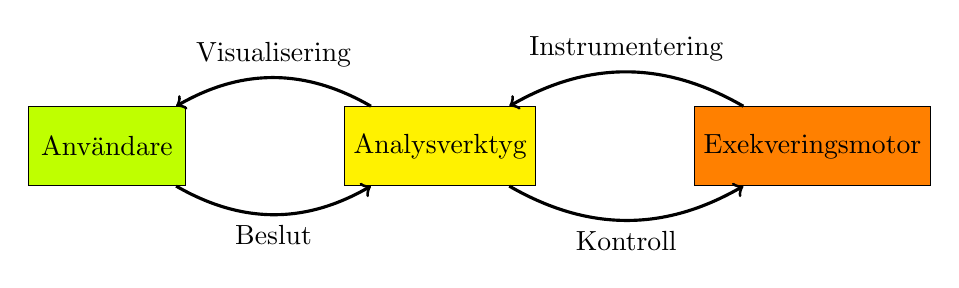
\begin{tikzpicture} \node [draw, fill=lime, minimum
	width=2cm, minimum height=1cm, ]  (user) {Användare};

		\node [draw, fill=yellow, minimum width=2cm, minimum height=1cm,
		right=2cm of user ] (tool) {Analysverktyg};

		\node [draw, fill=orange, minimum width=2cm, minimum height=1cm,
		right=2cm of tool ] (engine) {Exekveringsmotor};

		\draw[->, line width=.4mm] (user.-30) to[out=-30, in=-150]
		node[midway,below]{Beslut} (tool.-150);

		\draw[->, line width=.4mm] (tool.150) to[out=150, in=30]
		node[midway,above]{Visualisering} (user.30);

		\draw[->, line width=.4mm] (tool.-30) to[out=-30, in=-150]
		node[midway,below]{Kontroll} (engine.-150);

		\draw[->, line width=.4mm] (engine.150) to[out=150, in=30]
		node[midway,above]{Instrumentering} (tool.30);

	\end{tikzpicture} \caption{ Schematisk bild av ett binäranalysverktyg byggt
	kring en exekveringsmotor }\label{schematic} \end{figure}

\subsection{Analyser}

Det finns många möjliga analyser som kan användas av ett binäranalysverktyg, där
\textit{analyser} avser en visualisering av en aspekt av det analyserade
programmets beteende eventuellt inklusive ett sätt för användaren att påverka
det analyserade programmets körning.

En konkret exekvering kan spåras och dess instruktionssekvens kan visas för
användaren med loopar identifierade. Flera exekveringar kan visualiseras på
samma sätt och deras instruktionssekvenser användas för att återskapa
kontrollflödesstrukturer som for- och while-loopar och if-satser.

Möjligheter för \textit{state merging} kan identifieras helautomatiskt eller av
användaren, alltså platser där flera exekveringar kan ersättas av en enda mer
generell exekvering som innehåller ursprungsexekveringarnas skillnader som
symboliska uttryck.

En uppsättning liknande exekveringar kan visas upp för användaren tillsammans
med information om när och hur de divergerar, för att till exempel avgöra när
olika delar av indatan används.

För analys av programmet är det också hjälpsamt för användaren att kunna stega
genom exekveringen steg för steg och ändra på värden för att ta de vägar de vill
analysera. Detta borde också kunna göras baklänges, det vill säga att användaren
väljer en slutdestination och låter programmet själv lista ut vilka värden som
behövdes läsas för att exekveringen skulle ta sig till den punkten.

En mer automatisk men ändå viktig funktionalitet är konstruktion av kod-täckande
indata. När testfall som besöker en uppsättning instruktioner är konstruerad kan
kraven på indatan över denna uppsättning programhopp analyseras och programmet
kan lista ut vilka aspekter av indatan som kan ändras utan att påverka
kodtäckningsgraden, och kommunicera detta till användaren.

Det finns många möjliga analyser. Användbarheten i ett verktyg mäts inte i
kvantiteten analyser utan i förmågan för de utvalda implementerade analyserna
att täcka användarens behov av förståelse av programmet.


\section{Avgränsningar}
Att skapa en emulator är tidskrävande, dessutom är den resulterande produktens
korrekthet inte tillförlitlig utan nogrann testning. För att fastställa
korrekthet ska applikationen därför utnyttja existerande verktyg för att
exekvera programmet med stöd för symbolisk exekvering. Detta möjliggör också
bredare plattformssupport jämfört med en hemmasnickrad emulator.

\subsection{\stoe}

\stoe\cite{s2e} är en plattform för symbolisk exekvering som bygger på QEMU:s
virtuella maskin och använder KLEE\cite{klee}, en motor för symbolisk
exekvering, som interpreter för att möjliggöra symbolisk exekvering. \stoe\ är i
sin tur utbyggbart med möjlighet för användaren att skriva ett eget plugin för
att utföra analyser och används inom säkerhetsforskning för att till exempel
analysera skadlig kod. \stoe\ användes som del av Galactica-systemet som spelade
i DARPA Cyber Grand Challenge\cite{s2e_website}. \stoe\ är öppen källkod,
väldokumenterat och underhålls aktivt.

\subsection{SymQEMU}

Ett alternativt verktyg för symbolisk exekvering är symQEMU\cite{symqemu},
som också kombinerar QEMU:s virtuella maskin med KLEE:s motor för symbolisk
exekvering. Till skillnad från \stoe\ kompilerar SymQEMU KLEE in i den
analyserade binären och har jämförelsevis hög prestanda. Däremot har SymQEMU
bristfällig dokumentation och är ej aktivt uppdaterat.

\subsection{Beslut}

Då SymQEMU ej uppdateras aktivt och har bristfällig dokumentation kommer \stoe\
användas. Projektet avgränsas i och med att existerande verktyg (\stoe) kommer
användas istället för att bygga en motor för symbolisk exekvering från grunden.

\subsection{Konsekvenser}

Att använda \stoe\ innebär att arbetet avgränsas till att skapa ett plugin som
bygger ut motorn. Varken emulator eller motor ska byggas och de uppgifter som
ingår i att skapa en exekveringsmotor exkluderas.

Avgränsningen medför dessutom att fokus flyttas ifrån motorns tekniska detaljer
till att utveckla en användbar slutprodukt som bygger ut \stoe:s redan
existerande funktionalitet med ett grafiskt användargränsnitt och möjlighet att
stega igenom, analysera och interaktivt besluta om värden under exekvering.

Beslutet innebär att applikationens utformning blir bunden till \stoe:s tekniska
begränsningar.


\section{Metod/Genomförande}
Det är inte självklart hur utvecklingen av verktyget ska gå till och vilka
förmågor applikationen ska förses med för att uppfylla syftet. I det här
avsnittet beskrivs strategi och tillvägagångssätt för utvecklingen.

\subsection{Val av strategi}

För att uppnå och redogöra för möjligheterna i en potentiell applikation
reflekterades det över två möjliga alternativ att fullfölja. Dels diskuterades
alternativet att bygga en symbolisk exekveringsmotor från grunden och fokusera
på dess tekniska detaljer och dels att använda en existerande produkt där
fokuset istället ligger på att bygga plugin vars syfte är att utöka den
existerande motorn med fler funktioner.

Med syfte att göra framsteg valdes det att kolla vidare hur \stoe\ kan hjälpa i
frågan om att utöka funktionalitet i en existerande motor. \stoe\ är utvecklat
i programspråket C++ och med anledning av valet att utveckla i ett
annat programmeringsspråk, det vill säga Rust, krävs implementation av
C++-bindings. I ett första steg valdes det därför att se över hur detta går till
på lämpligt sätt och hur detta kan automatiseras med hjälp av andra verktyg
där bland annat autocxx ansågs som ett lovande alternativ.

\subsection{Tillvägagångssätt}
I avsikt att uppnå syftet med projektet, mer specifikt att utveckla ett
binäranalysverktyg, bestämdes det att ta fram demon som ska leda det
kontinuerliga utvecklingsarbetet.

Ett demo ska bestå av en analys med hjälp av verktyget som ökar förståelse för
ett exempelprogram. Exempelprogrammet ska ha som mål att visa en förmåga i
verktyget som underlättar förståelse för, eller belyser en känd intressant
egenskap hos exempelprogrammet. Exempelprogrammen ska skrivas i C eftersom
C-programs utseende i binärformat relativt väl motsvarar deras källkod. Detta
förenklar binäranalys och låter demot fokusera på sitt huvudämne. Dessutom ska
programmen vara så enkla som möjligt samtidigt som de uppnår sina mål.

Efter en framtagen id\'e för en demo och tillhörande exempelprogram, ska
verktyget utvidgas och utvecklas för att göra demot genomförbart.

Denna metod är önskad eftersom det tillåter att sätta uppnåbara delmål som styr
funktionaliteter som ska implementeras härnäst. Demon fungerar som test på dessa
funktionaliteter och visar att dessa är korrekta. Dessutom kan flera demon
utvecklas samtidigt vilket tillåter parallellism inom projektarbetet och
framsteg på flera fronter.

För att vidare kunna bestämma huruvida en demo är lämpligt och ska möjliggöras
genom utvidgning av verktyget kommer en avgränsning ske efter vad som är rimligt;
hur väl demots analysidé kan komma att tillämpas i verktyget och hur analysen
ökar användbarhet av verktyget. Dessutom ska det sättas i perspektiv till den tid
som krävs för att göra demot genomförbart med tanke på tidsramen för projektet.

I ett senare och/eller parallellt steg ska ett grafiskt användargränssnitt
utvecklas som tillåter användaren att traversera genom applikationen och göra
egna beslut gällande förgreningar av programmet etc. där användaren själv
bestämmer interaktivt nästa beslut som görs. Även detta arbetet styrs av demon
och funktionaliteter som önskas.

% Hur är detta kopplat till vårt syfte? Hur uppnår vi syftet med rapporten genom
% vald metod?

% (varför är typ besvarat i val av strategi-avsnittet)

% Hur besvarar vi huruvida valet av strategi är rimligt?

%


\section{Etiska och samhälleliga aspekter}
Beslutsanalysmodellen beskriven i \cite{foreskrifter} används för att bedöma om man behöver behöver ta hänsyn till samhälleliga eller etiska aspekter när problemställningen formuleras.
Analysen har tagit hänsyn till frågeställningarna
\begin{itemize}
    \item om vilka etiska aspekter som är relevanta för projektet;
    \item vilka nyttor eller etiska problem som kan uppkomma som ett resultat av projektets sannolika utfall; samt
    \item vilka parter som berörs av projektets utförande och projektets sannolika utfall.
\end{itemize}

En viktig etisk aspekt att ha i beaktande när man utvecklar verktyg som har som mål att underlätta sökandet efter säkerhetsbrister i programvaror är hur stor nytta verktyget är för \emph{försvarare} kontra \emph{attackerare}.
Med försvarare åsyftas de personer som har till uppgift att förhindra att ett datorsystem blir \emph{komprometterat}, medan attackerare har som mål att kompromettera datorsystem.
Att kompromettera ett datorsystem innebär att man på något sätt skadar ett datorsystems konfidentialitet; tillgänglighet; eller integritet.

Användandet av den typ av verktyg som planeras att utvecklas i projektet kommer inte att skiljas sig åt mellan försvarare och attackerare.
Medan försvararna använder verktygen för att hitta brister för att de ska veta vilka åtgärder de ska vidta för att höja säkerheten, använder attackerarna verktygen för att hitta brister som de sedan kan utnyttja för att påverka datorsystem negativt.

Personerna som berörs av projektet är främst attackerare och försvarare som får ännu ett verktyg för att genomföra dynamiska analyser av binärer.
Det anses inte vara ett problem om projektets slutprodukt är användbart, då det är vedertaget inom säkerhetssektorn att det är bättre att försvararna får bättre verktyg för att kunna utveckla nya säkerhetsmodeller; än att förhindra att attackerare får tillgång till bättre verktyg.
Om projektets slutprodukt inte anses användbart kommer projektet i realiteten inte ha någon etisk eller samhällelig påverkan.
Användarna av programvaror som analyseras av projektets slutprodukt kan påverkas om verktyget blir användbart för försvarare och attackerare, dels att fel i programvaran kan åtgärdas; men även att de kan utnyttjas av attackerare för att kompromettera användarna.


\section{Tidsplan}
Figur \ref{fig:tidsplan} visar en preliminär tidsplan för projektet och
aktiviteter för varje läsvecka. Alla externa datum och deadlines för inlämningar
är listade i tabell \ref{tab:deadlines}.


\begin{table}[h]
\caption{Datum och deadlines för viktiga aktiviteter}
\begin{center}
\begin{tabular}{| l | c |}
\hline
\bfseries{Aktivitet}                                 &  \bfseries{Datum} \\
\hline
Projektplan/Planeringsrapport                        &  2023-02-10\\
Muntlig halvtidsredovisning                          &  2023-03-07\\
Egen utvärdering 1                                   &  2023-03-12\\
Slutrapport, förgranskning                           &  2023-04-27\\
Sammanställd slutrapport                             &  2023-05-15\\
Bidragsrapport                                       &  2023-05-16\\
Film inlämning                                       &  2023-05-17\\
Skriftlig individuell opposition                     &  2023-05-22\\
Slutredovisning                                      &  2023-05-25/26\\
Egen utvärdering 2                                   &  2023-05-29\\
Slutlig inlämning av sammanställd slutrapport        &  2023-06-02\\
    \hline
\end{tabular}
\label{tab:deadlines}
\end{center}
\end{table}

\begin{figure}[htp]
\begin{center}

\newganttchartelement{foobar}{
    foobar/.style={
        shape=rectangle,
        inner sep=0pt,
        draw=gray!70!white,
        % draw=black,
        very thick,
        top color=gray!40,
        bottom color=gray!50,
        rounded corners=2pt
    },
    foobar incomplete/.style={
        /pgfgantt/foobar,
        draw=gray!70!white,
        top color=gray!30,
        bottom color=gray!10
    },
    foobar label font=\slshape,
}

\begin{ganttchart}[
        expand chart=\textwidth,
        y unit chart=0.9cm,
        foobar top shift=.3,
        foobar height=.7,
        vgrid={*{8}{gray, dotted}, *1{black, dashed}},
        title/.style={fill=gray, draw=none},
        title label font=\color{white}\bfseries,
        title height=1,
        progress=today,
        progress label text=\relax,
        today=4,
        milestone inline label node/.append style={rotate=30},
        milestone inline label node/.append style={left=2mm},
        milestone top shift=.45,
        milestone right shift=-.2,
        milestone left shift=0.3,
        foobar label font=\footnotesize,
    ]{1}{19}
    \gantttitle{LP 3}{9}        \gantttitle{LP 4}{9}        \gantttitle{}{1}\\
    \gantttitlelist{1,...,9}{1} \gantttitlelist{1,...,9}{1} \gantttitle{}{1} \\

    \ganttfoobar[inline]{Projektplan}{1}{4} \\

    % Eget
    \ganttfoobar[inline]{*\stoe-bygge}{2}{4} \\
    \ganttfoobar[inline]{*\stoe-infra}{3}{5} \\
    \ganttfoobar[inline]{*Demo-förslag}{5}{10} \\
    \ganttfoobar[inline]{*Demo-implementation}{5}{12} \\
    \ganttfoobar[inline]{*GUI-ramverk}{6}{11} \\ \\
    \ganttfoobar[inline]{*Slutprodukt}{8}{15} \\

    \ganttfoobar[inline]{Halvtidsredovisning}{6}{8} \\

    % TODO include deadlines for drafts of report for feedback meetings with fackspråk.
    \ganttfoobar[inline]{Film}{16}{17} \\
    \ganttfoobar[inline]{Skriftlig opposition}{17}{18} \\
    \ganttfoobar[inline]{Slutredovisning}{17}{18} \\

    \ganttfoobar[inline, foobar inline label node/.append style={left=2mm}]{Projektrapport}{5}{19}
    \ganttmilestone[inline]{Förgranskning}{14}{14}
    \ganttmilestone[inline]{Slutrapport}{16}{16}
    \ganttmilestone[inline]{Slutgiltig inlämning}{19}{19} \\

    \ganttlink{elem1}{elem2}
    \ganttlink{elem2}{elem4}
    \ganttlink{elem2}{elem6}
    \ganttlink{elem3}{elem4}
    \ganttlink{elem4}{elem6}
    \ganttlink{elem5}{elem6}

\end{ganttchart}
\end{center}
\caption{Tidsplan}
\label{fig:tidsplan}
\end{figure}

\subsection{Förklaring av aktiviteter i tidsplanen}

Tidsplanen i figur~\ref{fig:tidsplan} innehåller deadlines i italics,
administrativa och rapportrelaterade aktiviteter i normal stil och interna och
produktrelaterade aktiviteter har en stjärna * som prefix. Här följer en
förklaring av de produktrelaterade aktiviteterna:

\begin{labeling}{tidsplansbegrepp}

  \item [\textbf{\stoe-bygge}] Att etablera en miljö där \stoe:s huvudkomponent
    \texttt{libs2e.so} kan byggas reproducibelt och köras tillsammans med QEMU
    på en godtycklig binär, fast utan någon implementerad analys.

  \item [\textbf{\stoe-infra}] Att generera Rust-bindings till \texttt{libs2e.so}.
    Tooling för att kunna köra QEMU+\stoe\ med ett Rust-plugin på en testbinär.
    Viss abstraktion som gör det ergonomiskt att utveckla Rust-plugin:et.

  \item [\textbf{Demo-förslag}] Att skriftligt föreslå ett \textit{demo}, alltså
    en analys som kan implementeras ovanpå \stoe\ i form av ett program med
    specifikt syfte att genomföra en specifik sorts analys på små testprogram
    implementerade som enskilda C-filer.

  \item [\textbf{Demo-implementation}] Att implementera demon ovanpå \stoe, utan
    att integrera deras analyser till en sammanhängande enhet.

  \item [\textbf{GUI-ramverk}] Det kringarbete som krävs för att implementera
    analyser i allmänhet i slutprodukten, däribland det kringarbete som krävs
    för att bygga ett grafiskt gränssnitt.

  \item [\textbf{Slutprodukt}] Slutprodukten, med analyser härstammande från
    demon implementerade i en sammanhängande enhet.

\end{labeling}


\addcontentsline{toc}{section}{Referencer}
\bibliographystyle{plain} % We choose the "plain" reference style
\bibliography{refs} % Entries are in the refs.bib file

\end{document}
